\begin{pastexam}[label={px:ccu-111-swa-06}]{中正資工所甲組 111 學年度 第 14 題}
（單選）

(3\%) (\quad) The following is a list representation for a tree. The format of P(C1, C2)
in the representation represents that P is a parent node with two children nodes C1 and
C2.
\begin{center}( A ( B ( E ( K, L ), F ), C ( G ), D ( H ( M ), I, J ) ) )\end{center}
\begin{center}
\begin{tikzpicture}[x=0.9cm,y=0.9cm,>={Stealth[length=2mm]},font=\sffamily]
\newcommand{\pxlnode}[5]{% name, x, y, left, right
  \def\tmpa{#4}\def\tmpb{#5}%
  \ifx\tmpa\empty \draw[fill=gray!25] (#2,#3) rectangle ++(0.5,0.5);\else \draw (#2,#3) rectangle ++(0.5,0.5);\fi
  \ifx\tmpb\empty \draw[fill=gray!25] (#2+0.5,#3) rectangle ++(0.5,0.5);\else \draw (#2+0.5,#3) rectangle ++(0.5,0.5);\fi
  \node at (#2+0.25,#3+0.25) {#4}; \node at (#2+0.75,#3+0.25) {#5};
  \coordinate (#1-l) at (#2+0.25,#3+0.25); \coordinate (#1-r) at (#2+0.75,#3+0.25);
  \coordinate (#1-w) at (#2,#3+0.25); \coordinate (#1-n) at (#2+0.25,#3+0.5);}
% row 1
\pxlnode{A}{0.8}{0}{A}{} \pxlnode{P1}{2.5}{0}{}{} \pxlnode{P2}{7.05}{0}{}{} \pxlnode{P3}{10.05}{0}{}{0}
% row 2
\pxlnode{B}{2.5}{-1.7}{B}{} \pxlnode{P4}{4.0}{-1.7}{}{} \pxlnode{F}{5.4}{-1.7}{F}{0}
\pxlnode{C}{7.05}{-1.7}{C}{} \pxlnode{G}{8.45}{-1.7}{G}{0}
\pxlnode{D}{10.05}{-1.7}{D}{} \pxlnode{P5}{11.4}{-1.7}{}{} \pxlnode{I}{12.8}{-1.7}{I}{} \pxlnode{J}{14.2}{-1.7}{J}{0}
% row 3
\pxlnode{E}{4.0}{-3.4}{E}{} \pxlnode{K}{5.4}{-3.4}{K}{} \pxlnode{L}{6.75}{-3.4}{L}{0}
\pxlnode{H}{11.4}{-3.4}{H}{} \pxlnode{M}{12.8}{-3.4}{M}{0}
\foreach \a/\b in {A/P1,P1/P2,P2/P3,B/P4,P4/F,C/G,D/P5,P5/I,I/J,E/K,K/L,H/M} \draw[->] (\a-r) -- (\b-w);
\foreach \a/\b in {P1/B,P2/C,P3/D,P4/E,P5/H} \draw[->] (\a-l) -- (\b-n);
\end{tikzpicture}
\end{center}
Please draw this tree and convert it into a binary tree. What is the order of the nodes in
a post-order traversal of the binary tree?

a.~L, K, F, E, G, M, H, J, I, D, C, B, A \qquad b.~L, K, F, E, G, M, J, I, H, D, C, B, A\\
c.~K, L, F, E, G, M, H, J, I, D, C, B, A \qquad d.~K, L, F, E, G, M, J, I, H, D, C, B, A\\
e.~None of the above
\end{pastexam}

\begin{pastsoln}
答案是 b。

\textbf{讀圖。} 圖是這棵樹的廣義串列存法：每個串列節點兩格，右格指向同一層的下一個
節點（$0$ 是 \NIL）。 左格是字母的節點就是樹上的節點；左格灰色的節點表示這一項是一
棵子樹，左格指向那棵子樹的串列，串列的第一個是子樹的根，後面是它的子節點。 例如第
一列 $A$ 後面接了三個子樹項，分別指向以 $B$、$C$、$D$ 開頭的串列，所以 $A$ 有三個子
節點 $B, C, D$。 這和括號寫法一致，樹是
\[
A\bigl(B(E(K, L), F),\; C(G),\; D(H(M), I, J)\bigr).
\]

\textbf{轉成二元樹。} 用資結書第~7.2.3~節的左孩子右兄弟：第一個子節點當左子節
點，下一個兄弟當右子節點。
\begin{itemize}
\item $A$ 的左子節點 $B$；根沒有兄弟，右邊空。
\item $B$ 的左 $E$、右 $C$（$B$ 的下一個兄弟）；$C$ 的左 $G$、右 $D$；$D$ 的左 $H$、右空。
\item $E$ 的左 $K$、右 $F$；$K$ 的右 $L$。
\item $H$ 的左 $M$、右 $I$；$I$ 的右 $J$。
\end{itemize}
用資結書第~7~章的寫法是
$A\bigl(B(E(K(-, L), F),\; C(G, D(H(M, I(-, J)), -))),\; -\bigr)$：

\begin{center}
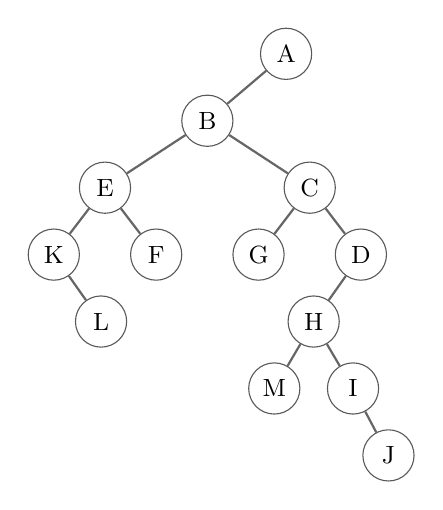
\begin{tikzpicture}[btn/.style={circle, draw=black!65, line width=0.4pt, minimum size=6.5mm, inner sep=0pt, font=\small},
    edge from parent/.style={draw=black!60, thick}, level distance=8.5mm,
    level 1/.style={sibling distance=20mm}, level 2/.style={sibling distance=26mm},
    level 3/.style={sibling distance=13mm}, level 4/.style={sibling distance=12mm},
    level 5/.style={sibling distance=10mm}, level 6/.style={sibling distance=9mm}]
\node[btn] {A}
    child {node[btn] {B}
        child {node[btn] {E}
            child {node[btn] {K} child[missing] child {node[btn] {L}}}
            child {node[btn] {F}}}
        child {node[btn] {C}
            child {node[btn] {G}}
            child {node[btn] {D}
                child {node[btn] {H}
                    child {node[btn] {M}}
                    child {node[btn] {I} child[missing] child {node[btn] {J}}}}
                child[missing]}}}
    child[missing];
\end{tikzpicture}
\end{center}

\textbf{後序。} 照「左子樹、右子樹、根」：
\begin{itemize}
\item $E$ 的子樹：$K$ 的子樹是 $L\;K$，再 $F$，再 $E$，得 $L\;K\;F\;E$。
\item $C$ 的子樹：$G$；$D$ 的子樹是「$H$ 的子樹、$D$」，$H$ 的子樹是 $M$、$J\;I$、$H$，
所以是 $M\;J\;I\;H\;D$；再 $C$。 得 $G\;M\;J\;I\;H\;D\;C$。
\item 接上 $B$、$A$：$L\;K\;F\;E\;G\;M\;J\;I\;H\;D\;C\;B\;A$，選 b。
\end{itemize}

其他選項：a 把 $H$ 放在 $J$、$I$ 前面，但 $I$、$J$ 在 $H$ 的右子樹裡，後序裡要排在 $H$
之前。 c、d 把 $K$ 放在 $L$ 前面，但 $L$ 是 $K$ 的右子節點，後序要先寫 $L$。 e 錯，因
為 b 對。 補充：這棵二元樹的\textbf{中序} $K\;L\;E\;F\;B\;G\;C\;M\;H\;I\;J\;D\;A$ 才是原
來那棵樹的後序（資結書第~7.2.3~節），二元樹的後序在原來的樹上沒有對應的意義，
作答時不要把兩者搞混。
\end{pastsoln}
